% !TEX root =./main.tex

\section{Block 7: Scan Conversion - Cometto}

Scan conversion handles the task of converting the stored beam data (in our case, in Mag\_image) from its polar reference (beam/sample or angle/distance) to a rectangular reference that can be used as data for an image.  Additionally, in order to form a continuous image, the values between the beams must be interpolated.

\subsection{Background}

Before discussing the implementation, we will first discuss the information necessary to understand and accomplish this task.  First, the signal data is stored in an array named \code{Mag\_image} where each row corresponds to a beam (angle), and each column corresponds to a sample (distance).  In our case, the array is $21 \times 4000$.  The output of the scan conversion stage is a $100 \times 201$ pixel image, which will be stored as a $100 \times 201$ array called \code{image}.

We will define the pixel at index $[1,101]$ as our position $(x,y) = (0,0)$.  From there, we can assign each pixel an angle, $\theta_p$, and a distance, $r_p$.  Then, we can perform bilinear interpolation using the equation
\begin{align*}
    \code{image[r,c]} = (1-\beta) &\left( (1 - \alpha) \code{Mag\_image[k,n]} + (\alpha) \code{Mag\_image[k+1,n]}  \right) \\ 
    + (\beta) &\left( (1-\alpha) \code{Mag\_image[k,n+1]} + (\alpha) \code{Mag\_image[k+1,n+1]} \right)
\end{align*}
with
\begin{align*}
    \alpha = \frac{\theta_p - \theta_k}{\theta_{k+1} - \theta_k}
\end{align*}
and
\begin{align*}
    \beta = \frac{r_p - r_n}{r_{n+1} - r_n}
\end{align*}
as the fractional offsets in the angle and distance directions, respectively.  This allows us to use use a weighted average of the four nearest known values to calculate the value at every pixel of the output image.

\subsection{Implementation}

In order to implement this algorithm in a fast way, we need to precompute as much as possible.  With the right values precomputed, it is possible to completely vectorize the function, as is done in \code{scan\_conversion.m}.  Ultimately, we need $8$ precomputed values, described in Table \ref{tab:precomputeScan}.

\begin{table}[H]
    \centering
    \begin{tabular}{cc}
        Parameter & Description  \\ \hline
        \code{ind\_bkn} & Set of linear indices for the $(k,n)$ value for each pixel \\
        \code{ind\_bk1n} & Set of linear indices for the $(k+1,n)$ value for each pixel \\
        \code{ind\_bkn1} & Set of linear indices for the $(n,k+1)$ value for each pixel \\
        \code{ind\_bk1n1} & Set of linear indices for the $(n+1,k+1)$ value for each pixel \\
        \code{BMAM} & The value of $(1-\beta)(1-\alpha)$ for each pixel \\
        \code{BMA} & The value of $(1-\beta)(\alpha)$ for each pixel \\
        \code{BAM} & The value of $(\beta)(1-\alpha)$ for each pixel \\
        \code{BA} & The value of $(\beta)(\alpha)$ for each pixel \\
    \end{tabular}
    \caption{Precomputed Values for Scan Conversion}
    \label{tab:precomputeScan}
\end{table}

To do these precalculations, we first need the distance and angle of each pixel.  To begin, we can calculate that the distance of each sample $n$ is given by
\begin{align*}
    r_n = \frac{nC}{2F_s}
\end{align*}
with $C = 1136 \text{ feet/s}$ and sampling frequency $F_s$.  We can also find that the angle of each beam $k$ is given by
\begin{align*}
    \theta_k = \arcsin(\frac{2kf_c}{F_s}) 
\end{align*}
for pulse frequency $f_c$.

With these, we can calculate the pixels per foot in the row ($y$) direction with
\begin{align*}
    \code{rppf} = \frac{\code{image\_rows}-1}{r_max}
\end{align*}
and in the column ($x$) direction with
\begin{align*}
    \code{cppf} = \frac{\code{image\_columns/2}-1}{r_max}
\end{align*}

Note here that a $100 \times 201$ pixel image has a ratio $\frac{\code{rppf}}{\code{cppf}}$ that is very close to one, which means that the output image is not distorted.

Finally, we can find the rectangular coordinates $(p_x, p_y)$ of the pixel at index $[p_r,p_c]$.  Noting that $(0,0)$ is at $[1,101]$ with
\begin{align*}
    p_x = \frac{(pc-101)}{\code{cppf}}
\end{align*}
and
\begin{align*}
    p_y = \frac{(pc-1)}{\code{rppf}}.
\end{align*}

Then, we can find the distance and angle of each pixel with
\begin{align*}
    r_p = \sqrt{p_x^2 + p_y^2}
\end{align*}
and
\begin{align*}
    \theta_p = \arctan(\frac{p_x}{p_y}).
\end{align*}

Finally, we can find the necessary indices.  The fractional indices of the pixel can be found with
\begin{align*}
    k_p = \frac{F_s \sin(\theta_p)}{2 f_c}
\end{align*}
and
\begin{align*}
    n_p = \frac{2F_sr_p}{C}.
\end{align*}

Then, we can round $n_p$ down (\code{floor}) for $n$, and add one for $n+1$.  Similarly, rounding $k_p$ down yields $k$, and adding one yields $k+1$.  Thus, we have the indices for our four neighboring points.  The last step is to convert $(row,column)$ indices to linear indices, which is done using the \code{sub2ind} script in \textsc{Matlab}.

Our second precomputational task is to find the fractional offset between the neighboring points.  The fractional offset in the $\theta$ direction is given by
\begin{align*}
    \alpha = \frac{\theta_p - \theta_k}{\theta_{k+1}-\theta_k},
\end{align*}
and we can calculate the fractional offset in the $r$ direction with
\begin{align*}
    \beta = \frac{r_p - r_n}{r_{n+1}-r_n}.
\end{align*}

Then, in order to vectorize the code, we can compute the four scaling factors for bilinear interpolation,
\begin{align*}
    (1-\beta)&(1-\alpha) \\
    (1-\beta)&(\alpha) \\
    (\beta)&(1-\alpha) \\
    (\beta)&(\alpha),
\end{align*}
for each point.  Thus, we have all $8$ of the necessary values that can be precomputed.  These are done in the \code{scan\_conversion\_precompute} function.

With all of these precalculations done, the calculation using the \code{Mag\_image} data can be done very quickly.  Implementing the bilinear interpolation calculation using the proper indexing, we have the simple and fast, single line that follows.

\begin{lstlisting}[language=Matlab]
    image=BMAM.*Mag_image(ind_bkn)+BMA.*Mag_image(ind_bk1n)...
        + BAM.*Mag_image(ind_bkn1) + BA.*Mag_image(ind_bk1n1);
\end{lstlisting}



\subsection{Development Process}

Before the analysis, we will briefly discuss the development process.  The design began by using a \code{for} loop to create a functional, yet not optizimied solution.  This enabled many bugs to be worked out before transitioning to the vectorized version.  Additionally, it laid the foundation for understanding and implementing the necessary precomputations.

\subsection{Test and Analysis}

In this stage, there are two main aspects that must be tested and analyzed.  First, we will confirm that the precomputations are performed correctly.  To do so, we will inspect Figure \ref{fig:scan_precompute}.

\begin{figure}[H]
    \centering
    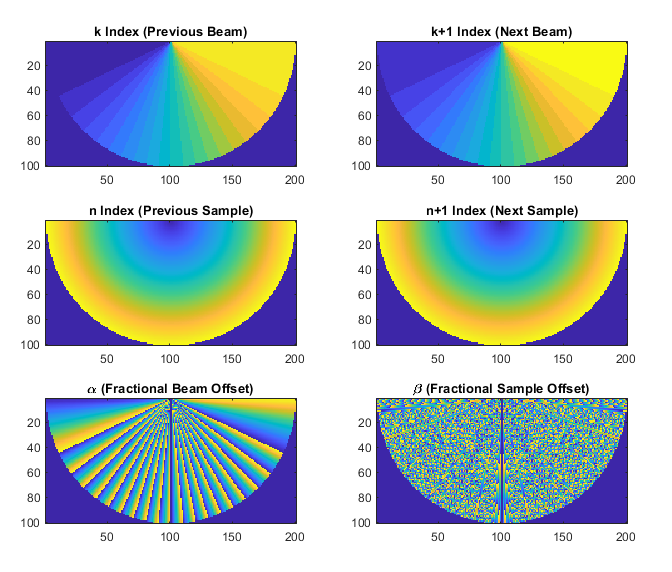
\includegraphics[width=0.8\linewidth]{figures/scan_precompute.png}
    \caption{Precomputation Plots by Image Pixel}
    \label{fig:scan_precompute}
\end{figure}

Notice that the data looks as expected.  First, we can see the previous and next beam indices sweep across the possible angles.  Additionally, the previous and next sample indices sweep through the distances.  Then, the fractional beam offset increases from zero as it gets closer to the next beam index.  The fractional sample offset does as well, though on a much smaller scale.  Thus, the precomputations were done successfully.

Next, we have three sets of synthetic data to confirm that the interpolation performs as intended.  First, we will transform and interpolate a block, as in Figure \ref{fig:scan_block}

\begin{figure}[H]
    \centering
    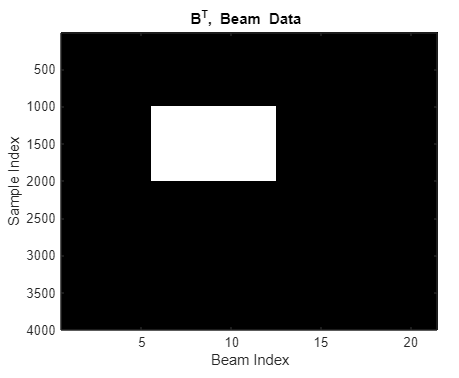
\includegraphics[width=0.5\linewidth]{figures/scan_block.png}
    \caption{Beam Data, Scan Test 1}
    \label{fig:scan_block}
\end{figure}

This beam data is successfully transformed, as can be seen in Figure \ref{fig:scan_block_out}.

\begin{figure}[H]
    \centering
    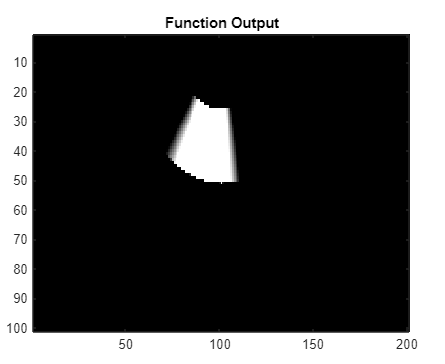
\includegraphics[width=0.5\linewidth]{figures/scan_block_out.png}
    \caption{Converted Image, Scan Test 1}
    \label{fig:scan_block_out}
\end{figure}

The next test, increasing in complexity, is with a double checkerboard, as can be seen in Figure \ref{fig:scan_checker2}.

\begin{figure}[H]
    \centering
    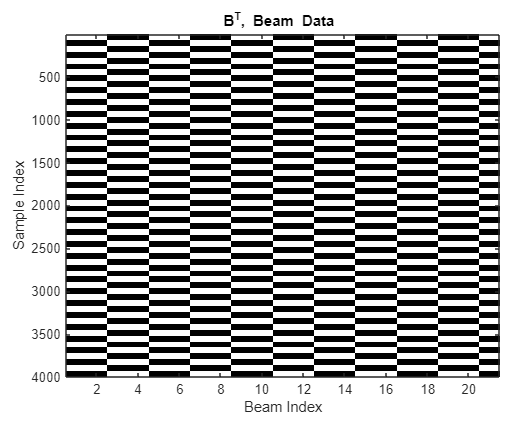
\includegraphics[width=0.5\linewidth]{figures/scan_checker2.png}
    \caption{Beam Data, Scan Test 2}
    \label{fig:scan_checker2}
\end{figure}

Again, this beam data is successfully transformed, as can be seen in Figure \ref{fig:scan_checker2_out}.

\begin{figure}[H]
    \centering
    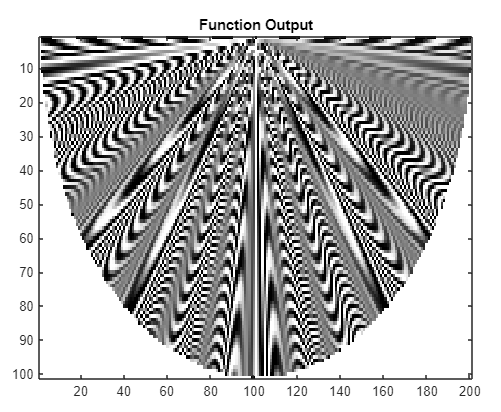
\includegraphics[width=0.5\linewidth]{figures/scan_checker2_out.png}
    \caption{Converted Image, Scan Test 2}
    \label{fig:scan_checker2_out}
\end{figure}

A third test is with a single, alternating checkerboard, as can be seen in Figure \ref{fig:scan_checker1}.

\begin{figure}[H]
    \centering
    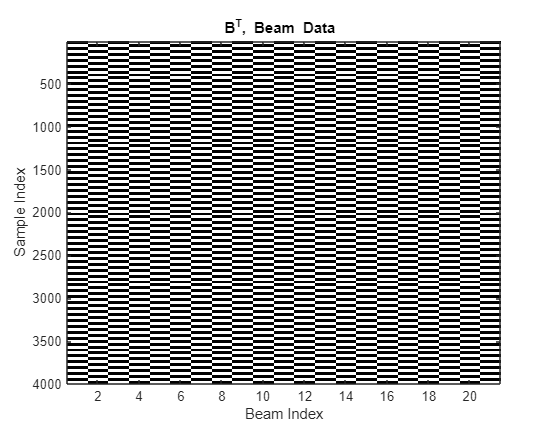
\includegraphics[width=0.5\linewidth]{figures/scan_checker1.png}
    \caption{Beam Data, Scan Test 3}
    \label{fig:scan_checker1}
\end{figure}

Again, this beam data is successfully transformed, as can be seen in Figure \ref{fig:scan_checker1_out}.

\begin{figure}[H]
    \centering
    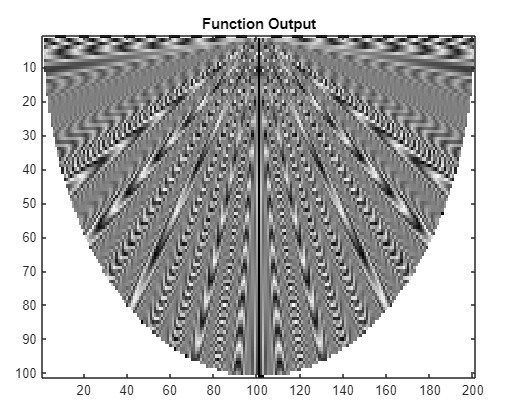
\includegraphics[width=0.5\linewidth]{figures/scan_checker1_out.png}
    \caption{Converted Image, Scan Test 3}
    \label{fig:scan_checker1_out}
\end{figure}

After conducting tests using synthetic data, we can further confirm using the real test data.  As can be seen in Figure \ref{fig:scan_real}, the system successfully interpolates real data as well.

\begin{figure}[H]
    \centering
    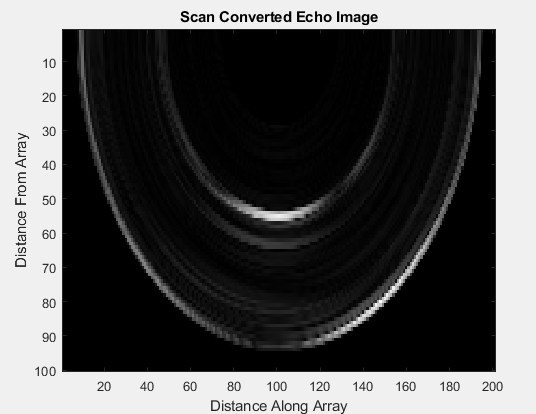
\includegraphics[width=0.5\linewidth]{figures/scan_real.png}
    \caption{Converted Image, Real Test Data}
    \label{fig:scan_real}
\end{figure}

The last aspect of the function to analyze is its timing.  Benchmarking is difficult, but here we are only comparing the newly written function to the provided \code{.p} file.  In this case, each function was timed (using \code{tic} and \code{toc}) over $10,000$ iterations, and the average runtimes can be seen in Table \ref{tab:scanConversionTime}.  The same data (the double checkerboard test pattern) was used, and the computer was in as similar a state as possible.  (Note, the provided \code{.p} function had a non-suppresed (no semicolon) line that outputted \code{max\_pixel = 10}, which needed to be suppressed using \code{evalc}, likely reducing the speed of the provided function.)

\begin{table}[H]
    \centering
    \begin{tabular}{cc}
        Function & Time ($\mu$s) \\ \hline
        Provided \code{.p} & $4002$\\
        Rewritten \code{.m} & $742.3$
    \end{tabular}
    \caption{Provided vs Rewritten Scan Conversion Performance}
    \label{tab:scanConversionTime}
\end{table}


As can be seen, the rewritten and vectorized \code{scan\_conversion.m} successfully interpolates and transforms the data into the correct format about 5 times faster than the provided function.  It is able to do this do to a substantial increase in precomputations. However, these precomputations only need to be calculated if certain configuration parameters are changed.  Thus, they are written to a file, and only incur precomputation time when necessary.